\documentclass[a4paper,12pt]{article}

\usepackage[a4paper,margin=2.2cm]{geometry}
\usepackage{amsmath,amssymb}
\usepackage{fontspec}
\usepackage{unicode-math}
\setmainfont{TeX Gyre Termes}
\setmathfont{TeX Gyre Termes Math}
\usepackage{graphicx}
\usepackage{booktabs}
\usepackage{float}
\usepackage{array}
\usepackage{tabularx}
\usepackage{xurl}
\usepackage[colorlinks=true,linkcolor=black,citecolor=black,urlcolor=blue]{hyperref}
\usepackage{setspace}
\usepackage{titlesec}
\usepackage{indentfirst}
\usepackage{fancyhdr}
\usepackage[nopatch=footnote]{microtype}
\usepackage{caption}
\usepackage{placeins}

\pagestyle{fancy}
\fancyhf{}
\cfoot{\thepage}
\renewcommand{\headrulewidth}{0pt}

\setlength{\parskip}{0.35em}
\setlength{\parindent}{2em}
\setlength{\emergencystretch}{1em}
\linespread{1.18}
\clubpenalty=10000
\widowpenalty=10000
\displaywidowpenalty=10000
\brokenpenalty=10000
\setlength{\abovecaptionskip}{5pt}
\setlength{\belowcaptionskip}{0pt}
\captionsetup{font=small,labelfont=bf}

\hypersetup{
  pdftitle={Social Pressure, Verified Turnout, and the Limits of Direct-Effect Interpretation},
  pdfauthor={Jiaquan Hong},
  pdfsubject={Design-aware reanalysis of a household-randomized voter-turnout field experiment},
  pdfkeywords={causal inference, randomized field experiment, voter turnout, randomization inference, interference}
}

\titleformat{\section}{\Large\bfseries}{\thesection}{0.8em}{}
\titleformat{\subsection}{\large\bfseries}{\thesubsection}{0.8em}{}

\title{Social Pressure, Verified Turnout, and the Limits of Direct-Effect Interpretation\\[4pt]
\large A design-aware reanalysis of a large household-randomized field experiment}
\author{Jiaquan Hong \quad Student ID: 23307110248}
\date{23307110248@m.fudan.edu.cn}

\begin{document}

\maketitle

\renewcommand{\abstractname}{\Large\bfseries Abstract}
\begin{abstract}
\vspace{4pt}
This note reanalyzes a large social-pressure voter-turnout field experiment using real administrative records from the Yale Dataverse. The archived file contains 344,084 voter records, 180,002 households, and 10,000 assignment blocks from the 2006 Michigan primary. The primary contrast compares assignment to a Neighbors mailer, which disclosed household and nearby voting histories, with no mailing. Verified turnout was 29.664 percent in control and 37.795 percent under Neighbors. The voter-level intention-to-treat effect is 8.131 percentage points, with a household-clustered standard error of 0.337 percentage points, a 99 percent confidence interval from 7.263 to 8.999, and a two-sided $p$-value of $2.41\times10^{-128}$. A household-level replication gives 8.479 percentage points, and block-stratified randomization inference with 999 draws gives a corrected $p$-value of 0.001. Adjustment, duplicate removal, balance checks, leave-one-block-out analysis, and observed-subgroup re-estimation preserve the conclusion. The four treatment arms form an ordered control-relative gradient, while a prespecified interaction analysis finds a 3.192 percentage-point larger effect among voters with higher prior-turnout propensity after Holm correction. The evidence does not identify every adjacent psychological mechanism or a spillover dose-response. Nearly all blocks have the same Neighbors saturation, so the defensible estimand is a household-assignment policy effect under possible interference rather than a pure individual direct effect. The result is statistically strong and policy-relevant, but external validity, privacy, autonomy, and reactance remain material limits.
\end{abstract}

\section{Question and contribution}

Social norms can alter participation even when the private instrumental value of one vote is small. A message that makes voting behavior observable may increase turnout by changing perceived civic duty, anticipated scrutiny, or reputational costs. The substantive importance of such an intervention depends on more than whether its average coefficient is nonzero. A credible analysis must establish the assignment unit, preserve the randomized comparison, quantify uncertainty at the appropriate dependence level, distinguish treatment bundles from mechanisms, and avoid treating public availability of voter records as a complete ethical justification.

This note studies how strongly assignment to increasingly intrusive social-pressure mailers changed verified turnout in the 2006 Michigan primary, whether the largest treatment effect is stable across reasonable design-based analyses, and which deeper interpretations remain unsupported. It uses the household-randomized experiment reported by Gerber, Green, and Larimer \cite{gerber2008}. The positive original result was public before the present analysis protocol was specified. The contribution is therefore neither discovery of an unknown treatment effect nor creation of another trial. It is a reproducible benchmark replication with explicit 99 percent uncertainty, household clustering, block-stratified randomization inference, multiplicity control, effect-modification tests, an interference-support audit, and a claim hierarchy that separates identified effects from appealing but unidentified explanations.

The principal finding is unusually large for a low-cost mobilization intervention. Assignment to the Neighbors mailer increases verified turnout by 8.131 percentage points relative to control, equivalent to a 27.4 percent increase over the control rate. The estimate changes little under block and baseline adjustment or exact-duplicate removal, and it remains positive in every reported observed subgroup. The ordered arm means also show that stronger disclosure is associated with larger effects. Yet the design does not independently vary exposure saturation within a block size. The main estimand must consequently be the policy effect of assigning a household to the mailer bundle under the realized experimental allocation, not a direct psychological effect holding every neighbor exposure fixed.

\section{Real-world data and experimental design}

\subsection{Provenance and outcome}

The data are real administrative voter records, not simulated voters or generated outcomes. The archived tab-separated file is distributed by the Yale Dataverse. Its persistent dataset identifier is \href{https://doi.org/10.60600/YU/CGMWNW}{DOI record}, \nolinkurl{10.60600/YU/CGMWNW}, and its data-file identifier is 42238. The local raw file contains 20,061,989 bytes and has SHA-256
\begin{center}
\small\path{05807BCBEDAACF02EC6E6838E1B9C9B2FC99AD9D8C63F80C162991970044C6CE}.
\end{center}
It contains 344,084 voter rows, 180,002 households, and 10,000 randomization blocks. The outcome records whether a registered voter actually voted in the August 2006 Michigan primary. It is administrative turnout rather than survey self-report. The prespecified analysis columns contain no missing values. The archive includes 119 exactly duplicated full rows; these are retained in the primary analysis because the raw archive is not silently altered and are removed only in a declared sensitivity analysis.

\begin{table}[H]
\centering
\caption{Data provenance and experimental design}
\label{tab:provenance}
\small
\setlength{\tabcolsep}{6pt}
\begin{tabularx}{0.96\textwidth}{lXl}
\toprule
Field & Recorded value & Analytical role \\
\midrule
Archive & Yale Dataverse & Institutional source \\
Dataset DOI & 10.60600/YU/CGMWNW & Persistent identifier \\
Data-file identifier & 42238 & Exact archived file \\
Voter rows & 344,084 & Administrative records \\
Households & 180,002 & Treatment-assignment unit \\
Assignment blocks & 10,000 & Stratified design \\
Primary outcome & Verified 2006 primary turnout & Binary administrative outcome \\
Treatment family & Four mailers and control & Ordered message bundles \\
\bottomrule
\end{tabularx}
\end{table}

\subsection{Assignment structure}

Households were assigned within blocks to control or to one of four mailed messages. The Hawthorne treatment informed recipients that their turnout was being studied. Civic Duty added a civic-participation appeal. Self displayed the household's own recent turnout history. Neighbors displayed the household's history and the histories of nearby households and indicated that updated records would follow the election. These arms are ordered bundles rather than separately randomized psychological ingredients. A contrast between two adjacent arms therefore identifies the effect of assignment to one complete message rather than the other, not a mediation pathway.

The dominant block contains 18 households: ten control households and two households in each active arm. This exact pattern occurs in 9,997 of 10,000 blocks. One other block of size 18 differs by one control-to-Hawthorne allocation, and two blocks of size 19 contain an additional Hawthorne or Civic Duty household. Household treatment labels are internally consistent. The primary voter-level Neighbors-control sample contains 229,444 records in 119,999 households: 191,243 control voters and 38,201 Neighbors voters.

\begin{figure}[!t]
\centering
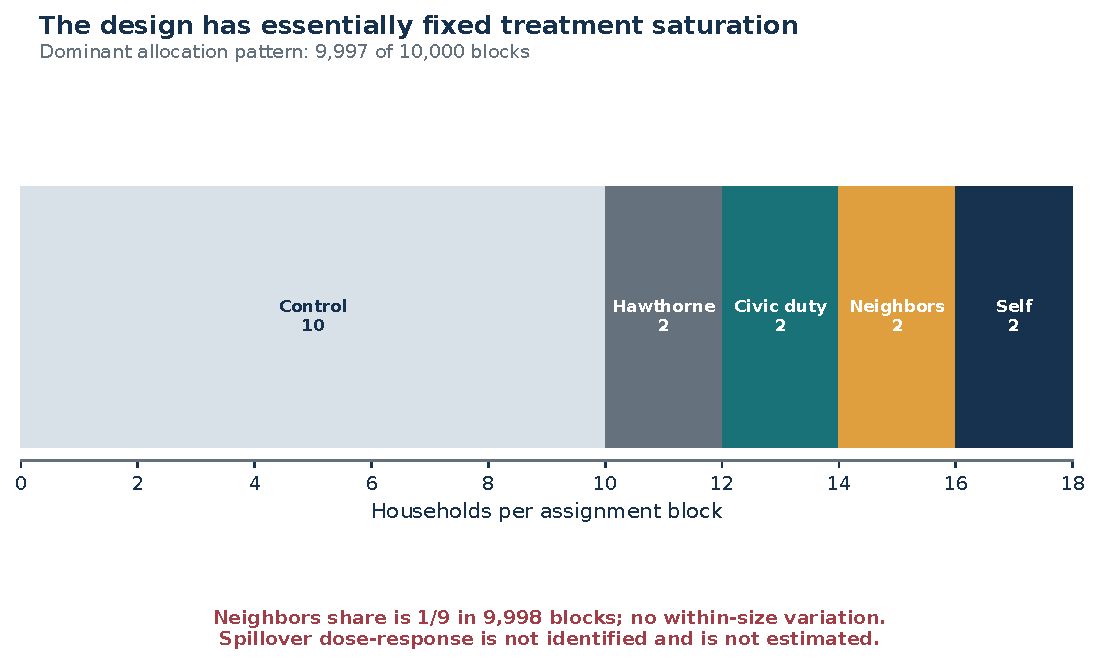
\includegraphics[width=0.96\textwidth]{../output/pdf/figure_4_design_interference.pdf}
\caption{The dominant block allocation and the resulting interference-support boundary. Treatment saturation is essentially fixed, so a Neighbors exposure dose-response is not identified.}
\label{fig:design}
\end{figure}

\section{Estimands and inference}

Let $Z_h$ denote assignment of household $h$ to the Neighbors mailer, and let $Y_{ih}$ denote verified turnout for voter $i$ in that household. The primary estimator is the difference in voter-level means,
\begin{equation}
\widehat\tau=\overline Y_{Z=1}-\overline Y_{Z=0}.
\end{equation}
Uncertainty is clustered by household because treatment is shared within a household and outcomes of co-resident voters need not be independent. The reported interval is
\begin{equation}
\widehat\tau \mathbin{\pm} t_{0.995,H-1}\widehat{\mathrm{SE}}_{\mathrm{cluster}},
\end{equation}
where $H$ is the number of observed households in the contrast. The 99 percent level makes the main interval more conservative than the conventional 95 percent interval and reduces reliance on a single significance threshold.

The adjusted specification includes randomization-block fixed effects and the prespecified baseline variables for prior general- and primary-election turnout, recorded sex, year of birth, and household size. Adjustment is used as a precision and stability check, not as a repair for failed randomization. A household-level replication averages turnout within each household and estimates the assignment contrast with one outcome per randomized unit. A duplicate sensitivity removes all exact duplicate full rows and repeats the primary voter-level estimator.

Randomization inference aggregates turnout to households and reassigns the observed treatment labels within each of the 10,000 blocks while preserving block-specific treatment counts. The observed statistic is the household-level Neighbors-control mean difference. With $B=999$ prespecified draws and $E=0$ draws at least as extreme as observed, the corrected two-sided Monte Carlo value is
\begin{equation}
p_{\mathrm{RI}}=\frac{1+E}{1+B}=0.001.
\end{equation}
This value is the resolution floor of the declared randomization exercise, not evidence that the randomization tail probability is exactly 0.001. The conventional clustered result, effect size, and randomization result should be read jointly.

The four control-relative treatment comparisons form one declared family and use Holm adjustment. Baseline-balance checks form another family. The secondary analysis tests four adjacent arm contrasts and three subgroup interactions with Holm correction within their declared families. Subgroup estimates alone are not treated as evidence of subgroup differences; interaction tests govern those claims.

\section{Main treatment effects}

Control turnout is 29.664 percent, compared with 37.795 percent under Neighbors. The primary effect is 8.131 percentage points. Its household-clustered standard error is 0.337 percentage points, the $t$ statistic is 24.13, and the 99 percent confidence interval is 7.263 to 8.999 percentage points. The two-sided clustered $p$-value is $2.41\times10^{-128}$. Statistical strength therefore rests on a large effect measured in more than 119,000 randomized households, not on a marginal crossing of a significance threshold.

The complete treatment family is ordered in the observed arm means. Relative to control, Civic Duty increases turnout by 1.790 percentage points, Hawthorne by 2.574, Self by 4.851, and Neighbors by 8.131. Every control-relative comparison remains significant after Holm adjustment. Figure~\ref{fig:gradient} reports household-clustered 99 percent intervals and makes the effect-size gradient visible without implying that the horizontal distance between adjacent arms is a separately randomized mediator.

\begin{figure}[!t]
\centering
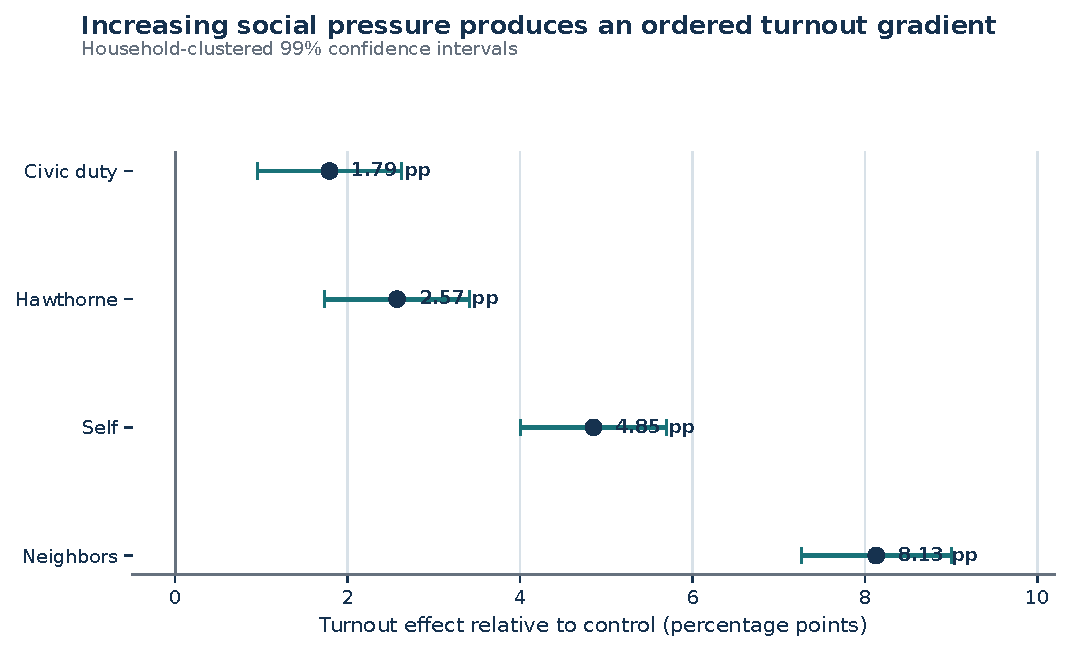
\includegraphics[width=0.96\textwidth]{../output/pdf/figure_1_pressure_gradient.pdf}
\caption{Control-relative turnout effects for the four mailed treatment bundles. Points are percentage-point estimates and bars are household-clustered 99 percent confidence intervals.}
\label{fig:gradient}
\end{figure}

\begin{table}[H]
\centering
\caption{Core Neighbors-control estimates}
\label{tab:core}
\small
\setlength{\tabcolsep}{4.5pt}
\begin{tabular}{lrrrrr}
\toprule
Estimator & Effect & SE & 99\% interval & $p$-value & $N$ \\
& \multicolumn{3}{c}{percentage points} & & \\
\midrule
Voter-level ITT & 8.1310 & 0.3370 & [7.2630, 8.9989] & $2.41\times10^{-128}$ & 229,444 \\
Block FE and baselines & 8.1465 & 0.2952 & [7.3862, 8.9068] & $3.72\times10^{-167}$ & 229,444 \\
Household-level outcome & 8.4788 & 0.3401 & [7.6027, 9.3549] & $8.07\times10^{-137}$ & 119,999 \\
Exact duplicates removed & 8.1253 & 0.3369 & [7.2574, 8.9932] & $3.53\times10^{-128}$ & 229,378 \\
Randomization inference & 8.4788 & -- & -- & 0.001 & 119,999 \\
\bottomrule
\end{tabular}
\end{table}

The adjusted estimate is 8.147 percentage points and the household-level estimate is 8.479. Removing the 119 exact duplicated rows changes the voter-level estimate by only $-0.0057$ percentage points. The different voter- and household-weighted estimands need not coincide because larger households receive more weight in the voter analysis. Their close magnitudes and identical substantive conclusions show that the result is not an artifact of one analytical level.

\section{Design diagnostics and robustness}

Random assignment should make pretreatment characteristics similar in expectation. Table~\ref{tab:balance} reports raw differences, standardized mean differences, and Holm-adjusted $p$-values for eight prespecified baseline variables. The largest absolute standardized difference is 0.0129 for 2004 primary turnout. Every Holm-adjusted value is at least 0.521. These diagnostics do not prove that every unmeasured feature is identical, but they show no material realized imbalance in the available baseline history.

\begin{table}[H]
\centering
\caption{Baseline balance for the primary Neighbors-control contrast}
\label{tab:balance}
\small
\setlength{\tabcolsep}{7pt}
\begin{tabular}{lrrrr}
\toprule
Baseline & Raw difference & Standardized difference & Raw $p$ & Holm $p$ \\
\midrule
General election 2002 & 0.00044 & 0.0011 & 0.851 & 1.000 \\
General election 2000 & -0.00172 & -0.0047 & 0.441 & 1.000 \\
Primary election 2004 & 0.00633 & 0.0129 & 0.065 & 0.521 \\
Primary election 2002 & -0.00279 & -0.0057 & 0.395 & 1.000 \\
Primary election 2000 & -0.00069 & -0.0016 & 0.815 & 1.000 \\
Recorded sex & 0.00112 & 0.0022 & 0.443 & 1.000 \\
Year of birth & -0.03939 & -0.0027 & 0.691 & 1.000 \\
Household size & 0.00410 & 0.0052 & 0.602 & 1.000 \\
\bottomrule
\end{tabular}
\end{table}

The outcome is observed for every record used in the primary comparison. All 10,000 blocks are informative for household-level randomization inference. A leave-one-block-out audit produces estimates from 8.1178 to 8.1420 percentage points, a total span of only 0.0242 percentage points. No individual assignment block drives the voter-level effect. Figure~\ref{fig:robustness} compares the prespecified estimators and observed subgroups using 99 percent intervals. Every interval excludes zero by a wide margin. The visible variation across subgroup point estimates motivates formal interaction testing rather than informal comparison of significance stars.

\begin{figure}[!t]
\centering
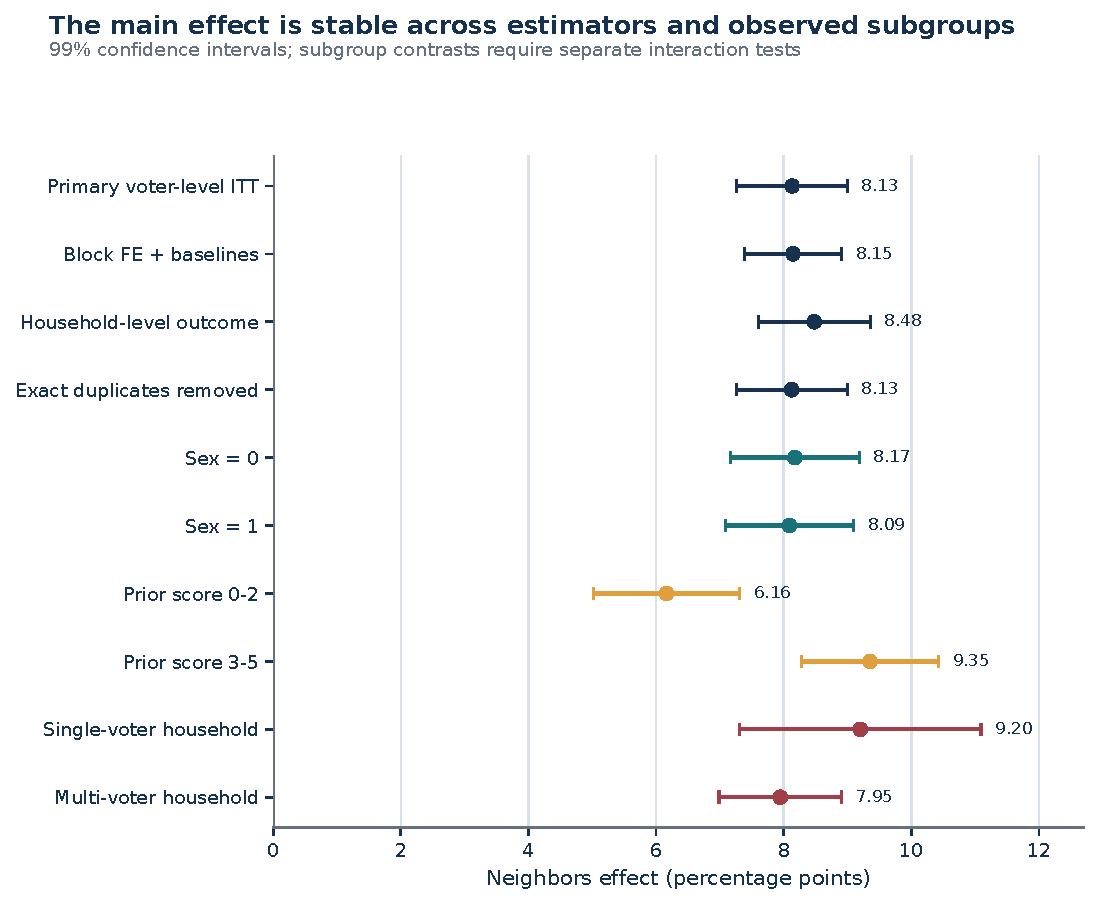
\includegraphics[width=0.96\textwidth]{../output/pdf/figure_3_robustness_forest.pdf}
\caption{Stability of the Neighbors effect across estimators and observed subgroups. Bars are 99 percent confidence intervals. Subgroup differences are governed by interaction tests rather than by visual comparison alone.}
\label{fig:robustness}
\end{figure}

The robustness evidence is deliberately redundant across inferential perspectives. Clustered regression uses a large-sample sampling approximation; household aggregation aligns the analysis with the randomized unit; block-stratified randomization inference relies on the known assignment mechanism; and leave-one-block-out analysis checks concentration. Their agreement substantially narrows the set of plausible computational or design-level explanations for the result.

\section{Effect modification and message contrasts}

Prior voting behavior is summarized by the number of recorded votes across five pretreatment elections. Figure~\ref{fig:heterogeneity} reports the Neighbors-control effect at scores zero through five. The estimates are 2.397, 5.871, 7.177, 9.532, 9.870, and 4.409 percentage points. All six control-relative effects remain significant after Holm adjustment, although the endpoints have smaller samples and wider intervals. The connected line is descriptive and is not a fitted dose-response curve.

\begin{figure}[!t]
\centering
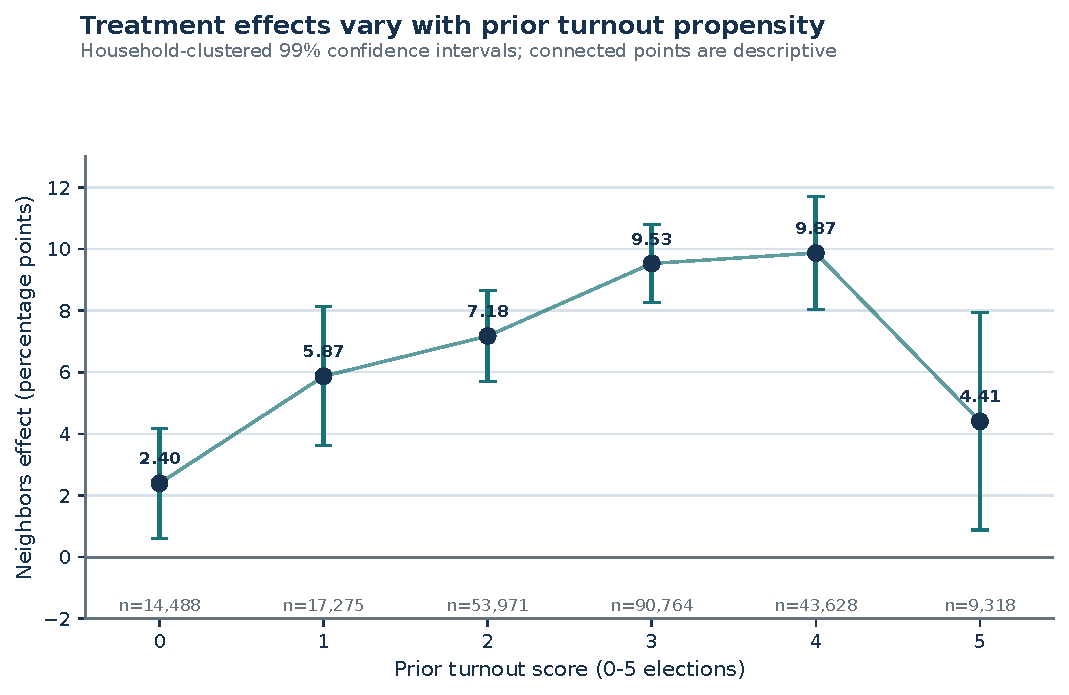
\includegraphics[width=0.96\textwidth]{../output/pdf/figure_2_prior_vote_heterogeneity.pdf}
\caption{Neighbors-control effects by pretreatment turnout score. Bars are household-clustered 99 percent confidence intervals; sample sizes appear below the points. The line is descriptive and no smooth functional form is assumed.}
\label{fig:heterogeneity}
\end{figure}

The prespecified primary interaction divides scores zero through two from scores three through five. The low-propensity effect is 6.162 percentage points and the high-propensity effect is 9.353, producing a 3.192 percentage-point interaction with household-clustered standard error 0.564. Its Holm-adjusted $p$-value is $4.57\times10^{-8}$. This is a statistically resolved effect-modification result within the study population. It does not establish whether the difference is caused by habit, social identity, baseline political interest, differential message attention, or another correlated feature.

Two other interactions are unresolved. Effects by recorded sex are 8.175 and 8.090 percentage points; their difference is $-0.085$ percentage points with Holm $p=0.831$. Effects in single- and multi-voter households are 9.202 and 7.947 percentage points; their 1.255 percentage-point difference has Holm $p=0.255$. The appropriate statements are that these differences were not resolved under the declared analysis, not that the treatment effects are proven equal.

The adjusted adjacent arm contrasts provide a separate check on the interpretation of the treatment gradient. Civic Duty exceeds control by 1.849 percentage points with Holm $p=5.31\times10^{-10}$. Hawthorne exceeds Civic Duty by 0.691 percentage points with Holm $p=0.066$. Self exceeds Hawthorne by 2.278 percentage points with Holm $p=3.54\times10^{-9}$, and Neighbors exceeds Self by 3.297 percentage points with Holm $p=6.13\times10^{-17}$. The overall ordering is strong, but the Hawthorne-Civic step is not resolved at conventional familywise levels. More importantly, each contrast compares complete messages. The data do not separately randomize observation, duty, self-disclosure, and neighbor disclosure as isolated mediators.

\section{Interference and the causal interpretation}

Standard individual potential-outcome notation often invokes no interference, under which one unit's outcome depends only on its own assignment. The Neighbors treatment makes this assumption substantively questionable because a mailed household receives information about other households and may itself be disclosed to others. When interference is possible, direct, indirect, total, and overall causal effects require explicit allocation programs and potential-outcome definitions \cite{hudgens2008}. Under general interference, identification further requires a design, a defensible exposure mapping, and exposure probabilities that support the target estimand \cite{aronow2017}.

The actual allocation does not support a Neighbors-saturation dose-response. Neighbors assignment equals two households in every block. Its share is $1/9$ in 9,998 blocks and $2/19$ in two blocks, but there is no distinct Neighbors share within either observed block size. Block size and share are therefore inseparable, and the two exceptional blocks provide no credible basis for a saturation analysis. A simulated allocation with richer saturation would describe a hypothetical new design, not add information to the observed experiment.

The primary comparison remains causally meaningful. It estimates the effect of assigning a household to the Neighbors mailer rather than control under the experiment's realized policy environment and allocation mechanism. That policy effect can include consequences of the bundled disclosure system. What it cannot do is hold every other household's exposure fixed and isolate a pure recipient-level psychological channel. The report consequently uses household-assignment policy ITT throughout. It records spillover as not identified, rather than interpreting the absence of an estimate as evidence of no spillover.

\section{External validity, persistence, and ethics}

The target context is a low-salience 2006 Michigan primary among registered voters included in the experiment. Later evidence helps assess relevance without converting the local estimate into a universal constant. Davenport and coauthors track more than one million voters from six social-pressure experiments and report statistically significant enduring effects in some elections one and sometimes two years later \cite{davenport2010}. Rogers and coauthors study social pressure in a high-salience election and find that the intervention remains consequential in a different electoral environment \cite{rogers2017}. A 17-state study involving 1.96 million citizens finds that social-pressure effects generalize across locations but vary with context, including election salience \cite{gerber2017}. These studies support a broader phenomenon while also showing why the Michigan estimate should not be transported mechanically to another state, election, year, or digital channel.

The large turnout effect is not itself a complete policy recommendation. Turnout history may be legally public while targeted household disclosure still changes practical privacy and perceived surveillance. Recipients in the original study contacted administrators, requested removal, and expressed objections, as summarized in the J-PAL evidence review \cite{jpal}. Related field experiments examine whether less aggressive social pressure or positive and negative social incentives can mobilize voters with different levels of reactance \cite{mann2010,panagopoulos2010}. A welfare comparison would need to value additional turnout alongside mailing costs, privacy loss, autonomy, complaints, administrative burden, and the availability of less intrusive alternatives.

The present data do not contain an individual welfare outcome, a validated privacy-cost measure, or a randomized comparison of implementation safeguards. They therefore support an effectiveness conclusion, not a net-benefit conclusion. Reporting the strong effect together with these costs is not a qualification forced by weak statistics. It is the distinction between estimating what the intervention changed and deciding whether institutions should deploy it.

\begin{table}[H]
\centering
\caption{Claim hierarchy after the design and literature audit}
\label{tab:claims}
\footnotesize
\setlength{\tabcolsep}{4pt}
\begin{tabularx}{0.98\textwidth}{>{\raggedright\arraybackslash}p{2.55cm} >{\raggedright\arraybackslash}p{2.65cm} >{\raggedright\arraybackslash}p{2.2cm} >{\raggedright\arraybackslash}X}
\toprule
Level & Claim & Status & Evidence boundary \\
\midrule
Primary & Policy ITT & Identified & Neighbors assignment versus control; verified turnout \\
Robustness & Stable effect & Supported & Adjustment, aggregation, duplicates, RI, and influence checks \\
Heterogeneity & Prior propensity & Supported & Interaction 3.192 pp; Holm $p=4.57\times10^{-8}$ \\
Heterogeneity & Sex or household size & Unresolved & Holm $p=0.831$ and 0.255 \\
Mechanism & Every adjacent component & Unresolved & Hawthorne-Civic Holm $p=0.066$; arms are bundles \\
Interference & Spillover dose-response & Not identified & No within-size Neighbors-saturation variation \\
Persistence & Later elections & External evidence & Not estimated from the current outcome \\
Transport & Universal 8.13 pp & Not identified & Local low-salience Michigan context \\
Welfare & Net desirability & Not established & Privacy, autonomy, reactance, and costs are unmeasured \\
\bottomrule
\end{tabularx}
\end{table}

\section{Reproducibility and audit trail}

The empirical workflow separates the untouched raw archive, prespecified protocols, executable analysis, machine-readable results, report figures, and publication output. The raw-file hash and schema are checked before analysis. The primary result, robustness audit, and mechanism analysis are stored as independent JSON artifacts. Figure generation reads those verified artifacts and writes both 300 dpi PNG and vector PDF versions. The build verifies the core result hashes and required figure files before compilation.

Negative and unresolved findings remain visible. The original positive result is disclosed as known before replication, the exact-duplicate issue is quantified, the Monte Carlo floor is labeled, and the interference analysis ends with non-identification rather than a synthetic substitute.

The report build compiles the source twice with XeLaTeX, checks for unresolved references and citations, rejects missing glyphs and layout warnings, and writes the stable artifact under \path{output/pdf}. Final verification renders every page with Poppler for visual inspection. This layered procedure is intended to make numerical provenance, inferential choices, and publication layout independently auditable.

\section{Conclusion}

The experiment provides a strong real-world causal result. In 119,999 households contributing to the primary comparison, assignment to the Neighbors social-pressure mailer increases verified turnout by 8.131 percentage points, with a household-clustered 99 percent confidence interval from 7.263 to 8.999 percentage points. Adjustment, household aggregation, exact-duplicate removal, block-stratified randomization inference, balance checks, and leave-one-block-out analysis support the same conclusion. The treatment family displays an ordered gradient, and the strongest mailer has a significantly larger effect among voters with higher prior-turnout propensity.

The same design discipline that strengthens the main conclusion limits deeper claims. One adjacent message contrast is unresolved, treatment bundles are not mediators, and fixed saturation prevents estimation of a spillover dose-response. The eligible conclusion is therefore a household-assignment policy effect under the realized experimental environment. Later studies support persistence and broader relevance, but the exact 8.13 percentage-point estimate remains local to the reported population and context. Privacy, autonomy, reactance, and administrative costs also prevent an effectiveness estimate from becoming an automatic policy endorsement.

This combination of a large effect and narrow interpretation is the central result. Statistical rigor does not require weakening a well-identified causal estimate. It requires stating precisely which decision the experiment randomized, which uncertainty the design supports, and which attractive explanations remain beyond the available evidence.

\footnotesize
\setlength{\parskip}{0.1em}
\begin{thebibliography}{9}
\setlength{\itemsep}{0pt}
\setlength{\parsep}{0pt}

\bibitem{aronow2017}
P. M. Aronow and C. Samii (2017).
\newblock Estimating average causal effects under general interference, with application to a social network experiment.
\newblock \href{https://doi.org/10.1214/16-AOAS1005}{\emph{Annals of Applied Statistics}}, 11(4), 1912--1947.

\bibitem{davenport2010}
T. C. Davenport, A. S. Gerber, D. P. Green, C. W. Larimer, C. B. Mann, and C. Panagopoulos (2010).
\newblock The enduring effects of social pressure: tracking campaign experiments over a series of elections.
\newblock \href{https://doi.org/10.1007/s11109-010-9122-0}{\emph{Political Behavior}}, 32(3), 423--430.

\bibitem{gerber2008}
A. S. Gerber, D. P. Green, and C. W. Larimer (2008).
\newblock Social pressure and voter turnout: evidence from a large-scale field experiment.
\newblock \href{https://doi.org/10.1017/S000305540808009X}{\emph{American Political Science Review}}, 102(1), 33--48.

\bibitem{gerber2017}
A. S. Gerber, G. A. Huber, A. H. Fang, and A. Gooch (2017).
\newblock The generalizability of social pressure effects on turnout across high-salience electoral contexts.
\newblock \href{https://doi.org/10.1177/1532673X16686556}{\emph{American Politics Research}}, 45(4), 533--559.

\bibitem{hudgens2008}
M. G. Hudgens and M. E. Halloran (2008).
\newblock Toward causal inference with interference.
\newblock \href{https://doi.org/10.1198/016214508000000292}{\emph{Journal of the American Statistical Association}}, 103(482), 832--842.

\bibitem{jpal}
Abdul Latif Jameel Poverty Action Lab (2026).
\newblock Social pressure and voter turnout in the United States.
\newblock \href{https://www.povertyactionlab.org/evaluation/social-pressure-and-voter-turnout-united-states}{J-PAL evaluation summary}.

\bibitem{mann2010}
C. B. Mann (2010).
\newblock Is there backlash to social pressure? A large-scale field experiment on voter mobilization.
\newblock \href{https://doi.org/10.1007/s11109-010-9124-y}{\emph{Political Behavior}}, 32(3), 387--407.

\bibitem{panagopoulos2010}
C. Panagopoulos (2010).
\newblock Affect, social pressure and prosocial motivation: field experimental evidence of the mobilizing effects of pride, shame and publicizing voting behavior.
\newblock \href{https://doi.org/10.1007/s11109-010-9114-0}{\emph{Political Behavior}}, 32(3), 369--386.

\bibitem{rogers2017}
T. Rogers, D. P. Green, J. Ternovski, and C. F. Young (2017).
\newblock Social pressure and voting: a field experiment conducted in a high-salience election.
\newblock \href{https://doi.org/10.1016/j.electstud.2017.02.004}{\emph{Electoral Studies}}, 46, 87--100.

\end{thebibliography}

\end{document}
